\documentclass[10pt,letterpaper]{article}
\usepackage[top=0.85in,left=2.75in,footskip=0.75in,marginparwidth=2in]{geometry}
\usepackage{listings}

% use Unicode characters - try changing the option if you run into troubles with special characters (e.g. umlauts)

\usepackage[utf8]{inputenc}


% clean citations
\usepackage{cite}

% hyperref makes references clicky. use \url{www.example.com} or \href{www.example.com}{description} to add a clicky url
\usepackage{nameref,hyperref}

% line numbers
\usepackage[right]{lineno}

% improves typesetting in LaTeX
\usepackage{microtype}
\DisableLigatures[f]{encoding = *, family = * }

% text layout - change as needed
\raggedright
\setlength{\parindent}{0.5cm}
\textwidth 5.25in
\textheight 8.75in

% use adjustwidth environment to exceed text width (see examples in text)
\usepackage{changepage}

% adjust caption style

% remove brackets from references
\makeatletter
\renewcommand{\@biblabel}[1]{\quad#1.}
\makeatother

% headrule, footrule and page numbers
\usepackage{lastpage,fancyhdr,graphicx}
\usepackage{epstopdf}
\pagestyle{myheadings}
\pagestyle{fancy}
\fancyhf{}
\rfoot{\thepage/\pageref{LastPage}}
\renewcommand{\footrule}{\hrule height 2pt \vspace{2mm}}
\fancyheadoffset[L]{2.25in}
\fancyfootoffset[L]{2.25in}

% use \textcolor{color}{text} for colored text (e.g. highlight to-do areas)
\usepackage{color}

% define custom colors (this one is for figure captions)
\definecolor{Gray}{gray}{.25}

% this is required to include graphics
\usepackage{graphicx}

% use if you want to put caption to the side of the figure - see example in text
\usepackage{sidecap}

% use for have text wrap around figures
\usepackage{wrapfig}
\usepackage[pscoord]{eso-pic}
\usepackage[fulladjust]{marginnote}
\reversemarginpar

% document begins here
\begin{document}
\vspace*{0.35in}

% title goes here:
\begin{flushleft}
{\Large
  \textbf\newline{pyranges: efficient comparisons of genomic intervals in Python}
  % and arithmetic run length-encoding
}
\newline
% authors go here:
\\
Endre Bakken Stovner\textsuperscript{1},
Pål Sætrom\textsuperscript{1, 2},
\\
\bf{1} Department of
  Computer Science, Norwegian University
  of Science and Technology, Trondheim, 7013, Norway
\\
\bf{2} Department of Clinical and Molecular Medicine, Norwegian
  University of Science and Technology, Trondheim, 7013, Norway
\\
\bigskip
* endrebak85@gmail.com

\end{flushleft}

\section*{Abstract}

\textbf{Summary:} PyRanges is a high-performance datastructure for representing
and manipulating genomic intervals and their associated data in Python. It is
directly compatible with Python's wealth of data science libraries and is
therefore well suited for genomic analyses.

\textbf{Availability and Implementation:} PyRanges is available open-source under
the MIT license at https://github.com/endrebak/pyranges and documentation exists
at https://endrebak.github.io/pyranges/

\textbf{Contact:} endrebak85@gmail.com

\section*{Introduction}


Comparing sets of intervals is a fundamental task in genomics, and a few basic
operations allow for answering complex questions. Several popular command
line tools for this purpose exist, like bedtools
\cite{doi:10.1093/bioinformatics/btq033} and bedops
\cite{doi:10.1093/bioinformatics/bts277}. There is also a wrapper for bedtools
which allows easy use from Python \cite{doi:10.1093/bioinformatics/btr539}.

Since comparing sets of intervals is such a fundamental task, the datastructure
GenomicRanges for efficiently representing and operating on genomic intervals
was invented. This datastructure removes the need for library authors to come up
with their own custom, slow and hard to maintain solutions and allows them to
immediately begin solving their problem of interest. Indeed, in R, the
foundational GenomicRanges library \cite{10.1371/journal.pcbi.1003118} is used
for interval comparisons, and it is a cornerstone of genomics packages in the R
BioConductor \cite{Gentleman2004} project. The new Julia language
\cite{doi:10.1137/141000671} also has a package for GenomicRanges
\cite{Haverty2017}.

Python is the fourth largest programming language in the world, the largest
scripting language, and it is widely used in bioinformatics, yet Python lacks a
GenomicRanges implementation. The PyRanges library remedies this.

\section*{Methods}

PyRanges is a thin wrapper around genomic data contained in Pandas
\cite{mckinney-proc-scipy-2010} dataframes. This allows one to directly use
Python's wealth of libraries for scientific computing and plotting such as
SciPy, NumPy, scikit-learn, matplotlib and seaborn \cite{scipy},
\cite{oliphant-2006-guide}, \cite{scikit-learn}, \cite{Hunter:2007},
\cite{michael_waskom_2017_883859} on the data in PyRanges objects. However, the
PyRanges object is extended with many methods for subsetting and modifying it,
and for doing comparisons and queries with pairs of PyRanges. The most important
are shown in table \ref{tab1}. PyRanges includes readers for common file formats
in bioinformatics such as bed, bam and gtf. PyRanges also contains coverage
methods, which allows one to represent and do arithmetic on the coverage (or
some other numeric score associated with each nucleotide) in an extremely
efficient manner. The coverage is stored as run length encodings in an object
called PyRles.

\section*{Functionality}

% TODO: find way to group

\begin{table}[!ht]
\begin{adjustwidth}{-1.5in}{0in}
\centering
\caption{{\bf Functionality.} Methods available on PyRanges objects.}
\begin{tabular}{|l|l|l|l|l|l|l|}
\hline
  {\bf Method} & {\bf Purpose} \\ \hline
  Subset & Use Python's getitem operator to efficiently subset PyRanges \\ \hline
  Intersection & For each feature in self, keep those that overlap with intervals in other \footnotemark \\ \hline
  Set Intersection & Treat the intervals in each PyRanges as a set and find the intersection \footnotemark \\ \hline
  Overlap & Keep each feature in self that overlaps with at least one in other \\ \hline
  Set Union & Treat the intervals in each PyRanges as a set and find the union \\ \hline
  Subtract & For each feature in self, keep those parts that do not overlap with any feature in other \\ \hline
  Set Subtract & Treat the intervals in each PyRanges as a set and subtract other from self \\ \hline
  Nearest & For each feature in self, find the nearest in other \\ \hline
  Cluster & Merge the overlapping features in a PyRanges object \\ \hline
  Coverage & Create a dictionary of run length encodings from the PyRanges object \\ \hline
\end{tabular}
\label{tab1}
\end{adjustwidth}
\end{table}
\footnotetext{Like bedtools intersect}
\footnotetext{Like BioConductor GenomicRanges intersect}


\subsection*{Implementation}

PyRanges are stored in Pandas DataFrames, which are 2-D, mutable representations
of data. To allow for range-queries and operations that uses such, the genomic
intervals are stored in a nested containment list, originally implemented in the
PyGr library \cite{doi:10.1093/bioinformatics/btl647}.

\section*{Performance}

The PyRanges library has been extensively tested for both speed and memory use.
In the below tests, sorted files were used. This does not affect the runtime or
memory-usage of PyRanges/GenomicRanges, but makes PyBedTools faster and less
memory-consuming. As PyBedTools always reads and writes for each operation, it
is impossible to measure purely the speed of the operation in PyBedTools.

\subsection*{Speed}

PyRanges was tested against GenomicRanges and PyBedtools for speed, shown in
figure \ref{fig1}, and memory usage, shown in figure \ref{fig2}. For object
instantiation, PyRanges is a bit slower than GenomicRanges, but for the
operations themselves PyRanges is up to twice as fast. We see that PyBedTools
matches the speed of the R and Python GenomicRanges-implementations as it can
use the extremely efficient sweep algorithm. For most other algorithms we see
that it uses a lot more time, however.

\begin{figure}
% the number in [] of wrapfigure is optional and gives the number of text lines that should be wrapped around the text. Adjust according to your figures height
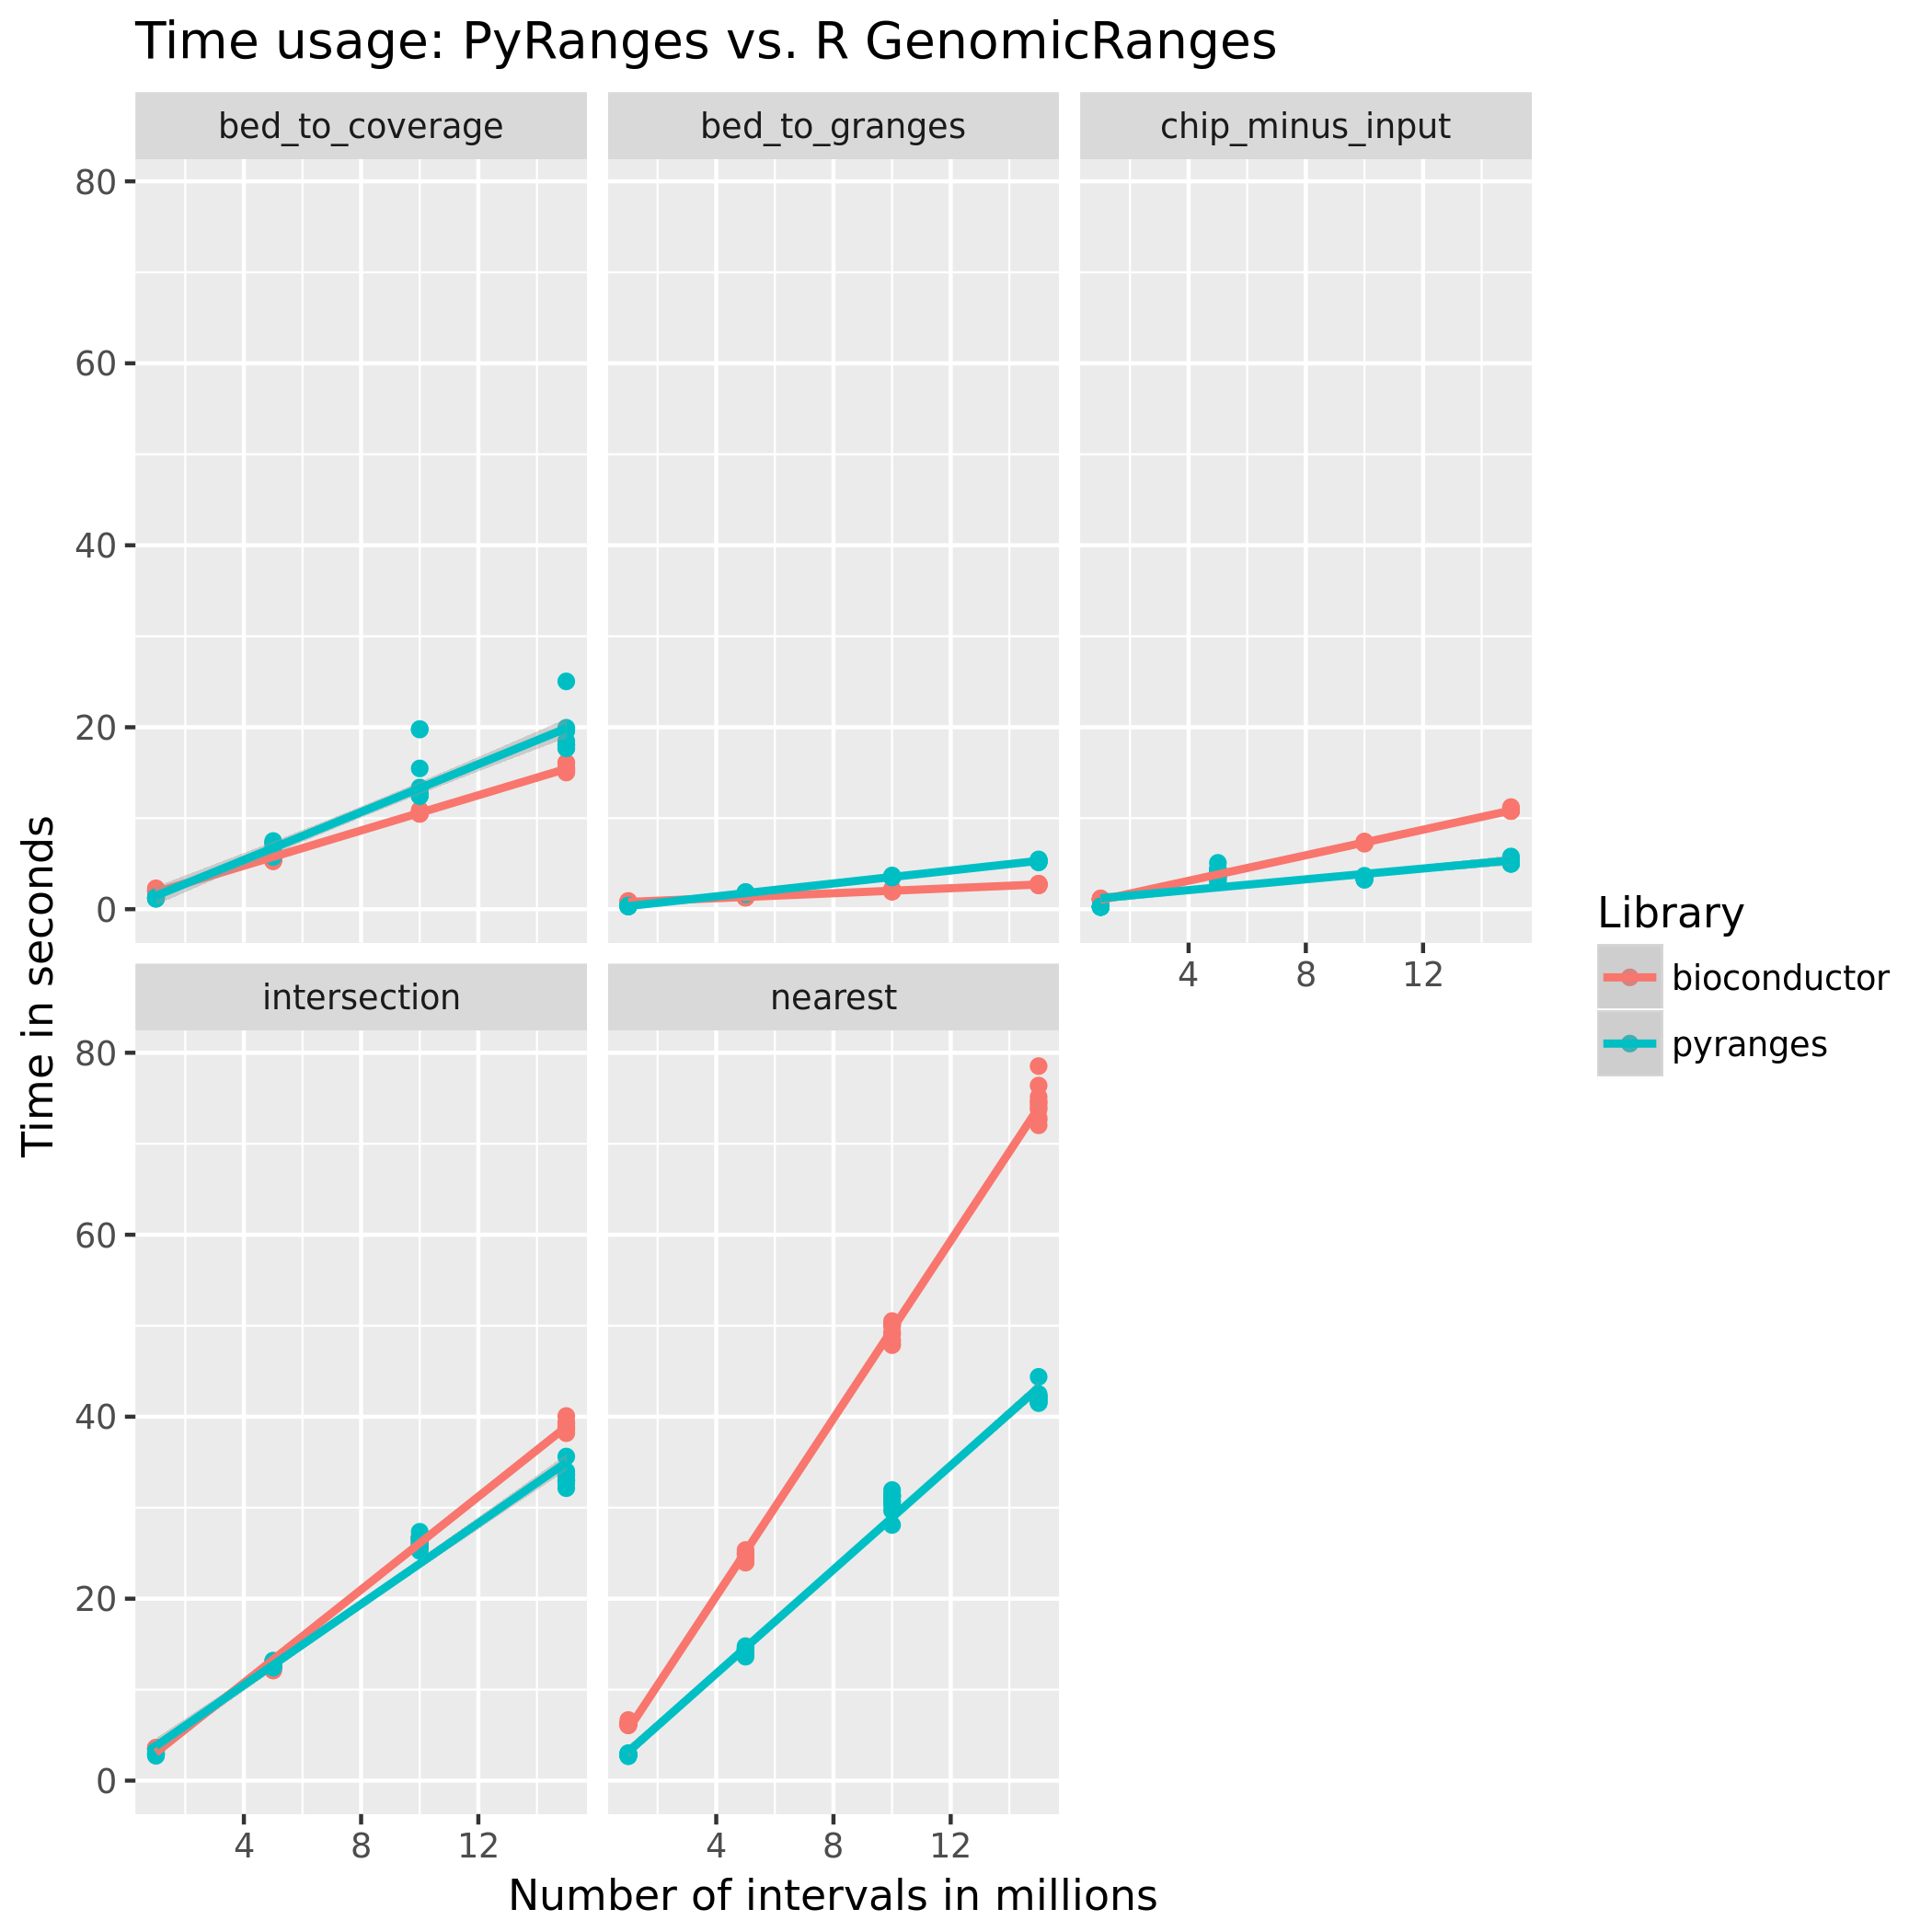
\includegraphics[width=1\textwidth]{graphs/time.pdf}
% \captionsetup{labelformat=empty} % makes sure dummy caption is blank
\caption{Time in seconds: PyRanges vs. GenomicRanges} % add dummy caption - otherwise \label won't work and figure numbering will not count up
\label{fig1} % use \ref{fig1} to reference to this figure
\end{figure} % avoid blank space here

\subsection*{Memory usage}

Memory usage of the PyRanges library was tested using the benchmarking
capabilities of Snakemake \cite{doi:10.1093/bioinformatics/bty350}. It works by
polling the running process, which means that the estimates for memory usage
also includes setup.

For most functionality, PyRanges uses a bit less memory than GenomicRanges. The
only cases where PyRanges uses more memory is for rle arithmetic and nearest,
where PyRanges leverages this memory to make the operations much faster
than R GenomicRanges. There is some variability in the memory usage, which is to
be expected for garbage collected languages. We see that pybedtools is extremely
memory-efficient for many operations.

\begin{figure}
% the number in [] of wrapfigure is optional and gives the number of text lines that should be wrapped around the text. Adjust according to your figures height
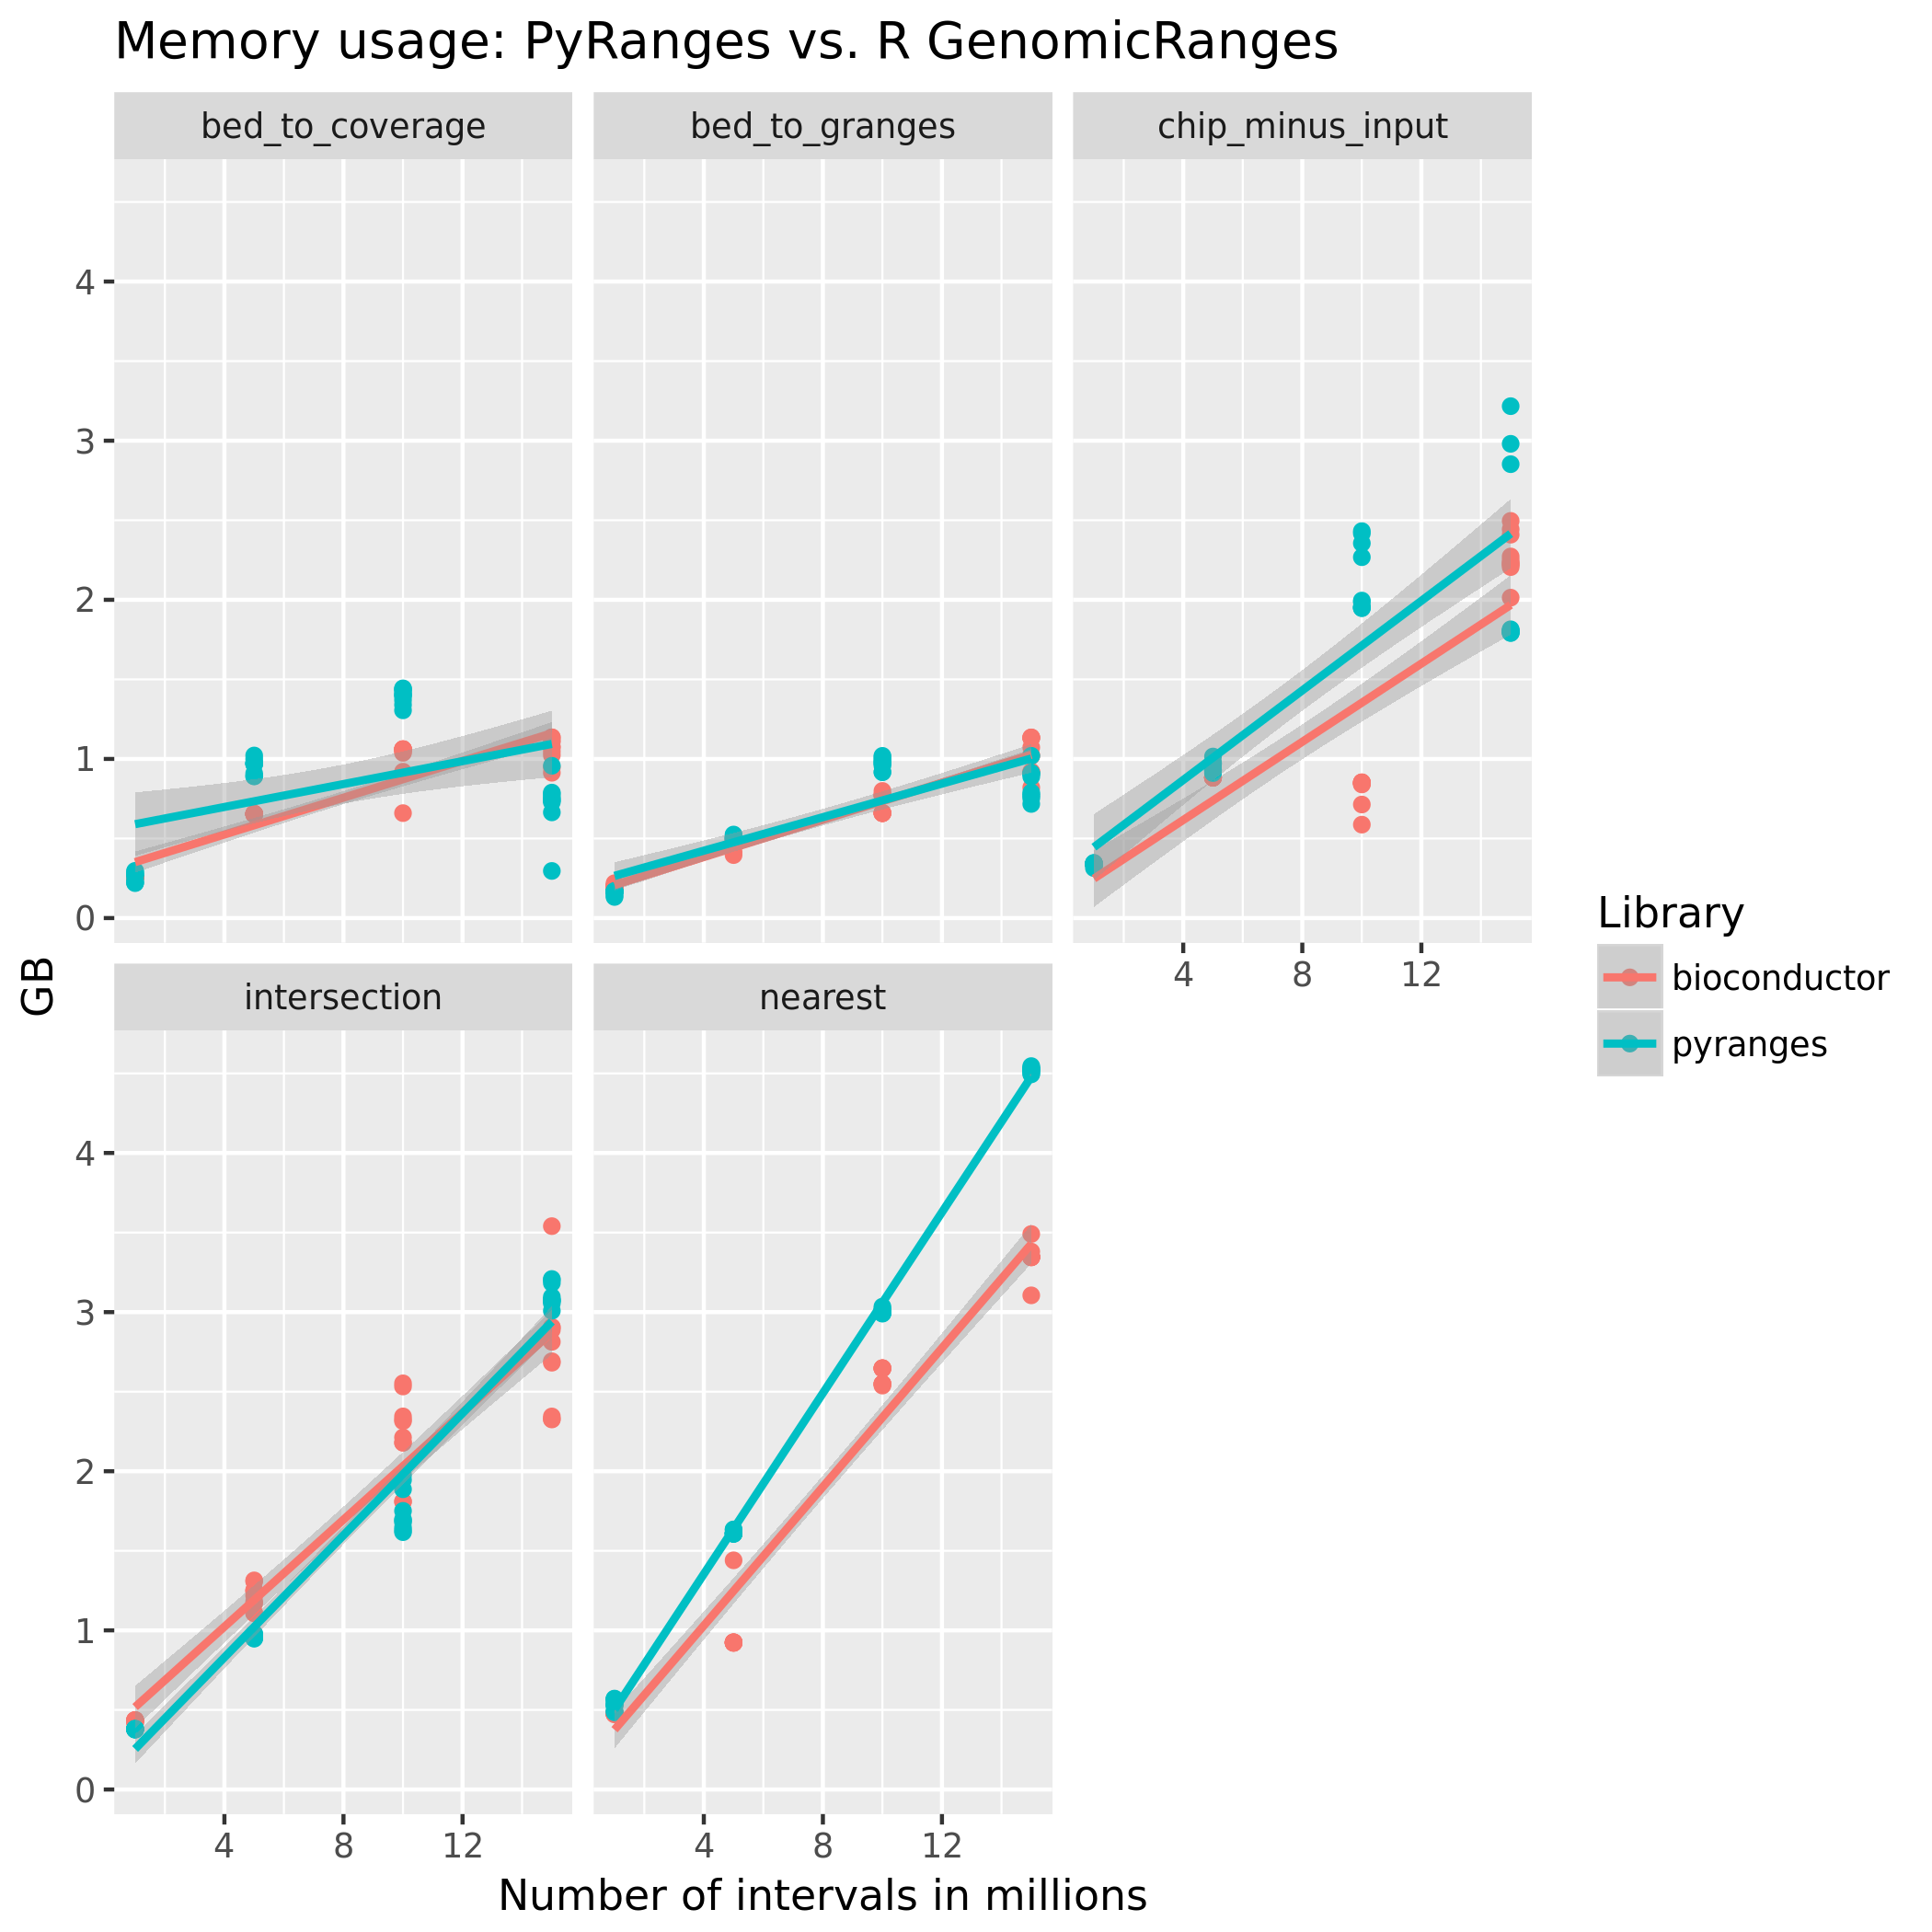
\includegraphics[width=1\textwidth]{graphs/memory.pdf}
% \captionsetup{labelformat=empty} % makes sure dummy caption is blank
\caption{Memory usage in GigaBytes: PyRanges vs GenomicRanges} % add dummy caption - otherwise \label won't work and figure numbering will not count up
\label{fig2} % use \ref{fig1} to reference to this figure
\end{figure} % avoid blank space here

\section*{Discussion}

PyRanges works well with the existing Python data science libraries yet extends
them with high-performance functionality for genomic analyses. As such we
believe it will be useful for everything from simplifying one-off analysis
scripts to providing a foundation for bioinformatics libraries written in
Python.


\bibliography{library}

\bibliographystyle{abbrv}

\end{document}


% \subsection*{Advantages}

% In contrast to PyRanges, which stores the data in memory, PyBedtools uses disk
% space for storing temporary results, which requires additional resource
% management by users and can lead to resource leaks; e.g. if the process calling
% PyBedtools is killed.

% PyBedtools: rigid in input format. If one operation merges reads and does not
% preserve all columns, then the file is not usable in further operations with
% bedtools.

% To make it go fast, need to sort. If already sorted, this is a waste of time.
% Often a bother; need to keep two copies of same file.

% Cannot do region-based lookups in bedfile easily.



% \section*{Example Usage}

% \begin{adjustwidth}{-2in}{0in}
% \begin{flushright}
% \begin{lstlisting}[language=Python, linewidth=30cm, basicstyle=\small]
%   import pyranges as pr
%   from pyranges import PyRanges

%   > gr1 = pr.read_bed('f1.bed')

%   +--------------+---------+-------+--------+---------+----------+
%   | Chromosome   |   Start |   End | Name   |   Score | Strand   |
%   |--------------+---------+-------+--------+---------+----------|
%   | chr1         |       3 |     6 | h      |       0 | +        |
%   | chr1         |       5 |     7 | h      |       0 | -        |
%   | chr1         |       8 |     9 | h      |       0 | +        |
%   +--------------+---------+-------+--------+---------+----------+
%   PyRanges object has 3 sequences from 1 chromosomes.

%   > gr2 = pr.read_bed('f2.bed')

%   +--------------+---------+-------+--------+---------+----------+
%   | Chromosome   |   Start |   End | Name   |   Score | Strand   |
%   |--------------+---------+-------+--------+---------+----------|
%   | chr1         |       1 |     2 | f      |       0 | +        |
%   | chr1         |       6 |     7 | f      |       0 | -        |
%   +--------------+---------+-------+--------+---------+----------+
%   PyRanges object has 2 sequences from 1 chromosomes.

%   > n = gr1.nearest(gr2, strandedness="opposite", overlapping=False, suffix='_')

%   # The PyRanges data can be accessed with .df
%   > n.df[["Chromosome", "Start", "End", "Strand", "Start_", "End_", "Strand_", "Distance"]]

%     Chromosome  Start  End Strand  Start_  End_ Strand_  Distance
%   0       chr1      3    6      +       6     7       -         1
%   1       chr1      8    9      +       6     7       -         2
%   2       chr1      5    7      -       1     2       +         4

%   # Easily create new PyRanges from a df

%   > PyRanges(n.df[["Chromosome", "Start", "End", "Strand", "Start_", "End_", "Strand_", "Distance"]])

%   +--------------+---------+-------+----------+----------+--------+-----------+------------+
%   | Chromosome   |   Start |   End | Strand   |   Start_ |   End_ | Strand_   |   Distance |
%   |--------------+---------+-------+----------+----------+--------+-----------+------------|
%   | chr1         |       3 |     6 | +        |        6 |      7 | -         |          1 |
%   | chr1         |       8 |     9 | +        |        6 |      7 | -         |          2 |
%   | chr1         |       5 |     7 | -        |        1 |      2 | +         |          4 |
%   +--------------+---------+-------+----------+----------+--------+-----------+------------+
%   PyRanges object has 3 sequences from 1 chromosomes.

%   > gr1.intersection(gr2)

%   +--------------+---------+-------+--------+---------+----------+
%   | Chromosome   |   Start |   End | Name   |   Score | Strand   |
%   |--------------+---------+-------+--------+---------+----------|
%   | chr1         |       6 |     7 | h      |       0 | -        |
%   +--------------+---------+-------+--------+---------+----------+
%   PyRanges object has 1 sequences from 1 chromosomes.

%   > c = gr1.cluster()
%   > c

%   +--------------+---------+-------+
%   | Chromosome   |   Start |   End |
%   |--------------+---------+-------|
%   | chr1         |       3 |     7 |
%   | chr1         |       8 |     9 |
%   +--------------+---------+-------+
%   PyRanges object has 2 sequences from 1 chromosomes.

%   > c.df.insert(3, 'ID', ["A", "B"])
%   > c

%   +--------------+---------+-------+------+
%   | Chromosome   |   Start |   End | ID   |
%   |--------------+---------+-------+------|
%   | chr1         |       3 |     7 | A    |
%   | chr1         |       8 |     9 | B    |
%   +--------------+---------+-------+------+
%   PyRanges object has 2 sequences from 1 chromosomes.

%   > cv1 = gr1.coverage(strand=True)
%   > cv1

%   chr1 +
%   --
%   +--------+-----+-----+-----+-----+
%   | Runs   |   3 |   3 |   2 |   1 |
%   |--------+-----+-----+-----+-----|
%   | Values |   0 |   1 |   0 |   1 |
%   +--------+-----+-----+-----+-----+
%   Rle of length 9 containing 4 elements

%   chr1 -
%   --
%   +--------+-----+-----+
%   | Runs   |   5 |   2 |
%   |--------+-----+-----|
%   | Values |   0 |   1 |
%   +--------+-----+-----+
%   Rle of length 7 containing 2 elements
%   PyRles object with 2 chromosomes/strand pairs.

%   > cv2 = gr2.coverage(strand=True)
%   > cv2

%   chr1 +
%   --
%   +--------+-----+-----+
%   | Runs   |   1 |   1 |
%   |--------+-----+-----|
%   | Values |   0 |   1 |
%   +--------+-----+-----+
%   Rle of length 2 containing 2 elements

%   chr1 -
%   --
%   +--------+-----+-----+
%   | Runs   |   6 |   1 |
%   |--------+-----+-----|
%   | Values |   0 |   1 |
%   +--------+-----+-----+
%   Rle of length 7 containing 2 elements
%   PyRles object with 2 chromosomes/strand pairs.

%   > cv1 - cv2

%     chr1 +
%   --
%   +--------+-----+-----+-----+-----+-----+-----+
%   | Runs   |   1 |   1 |   1 |   3 |   2 |   1 |
%   |--------+-----+-----+-----+-----+-----+-----|
%   | Values |   0 |  -1 |   0 |   1 |   0 |   1 |
%   +--------+-----+-----+-----+-----+-----+-----+
%   Rle of length 9 containing 6 elements

%   chr1 -
%   --
%   +--------+-----+-----+-----+
%   | Runs   |   5 |   1 |   1 |
%   |--------+-----+-----+-----|
%   | Values |   0 |   1 |   0 |
%   +--------+-----+-----+-----+
%   Rle of length 7 containing 3 elements
%   PyRles object with 2 chromosomes/strand pairs.

% \end{lstlisting}
% \end{flushright}

% \end{adjustwidth}